\documentclass[../main/main.tex]{subfiles}


\begin{document}

\section{October  8th, 2020}
\subsection{Upwind and Lax-Wendroff Analysis}
The solutions to the upwind and Lax-Wendroff methods have different properties. For example:
\begin{figure}[h!]
\centering
\begin{subfigure}{.5\textwidth}
  \centering
  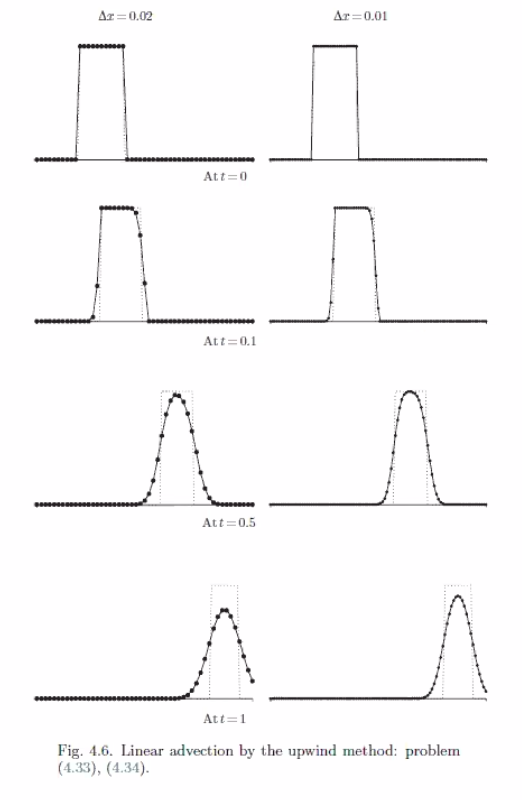
\includegraphics[width=.8\linewidth]{10-8upwind}
  \caption{Upwind Method}
  \label{fig:sub1}
\end{subfigure}%
\begin{subfigure}{.5\textwidth}
  \centering
  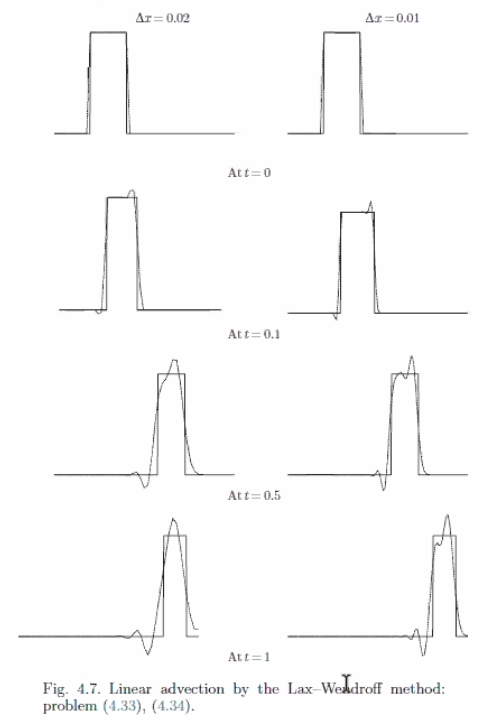
\includegraphics[width=.8\linewidth]{10-8lax}
  \caption{Lax-Wendroff Method}
  \label{fig:sub2}
\end{subfigure}
\caption{Modified Equation Analysis}
\label{fig:test}
\end{figure}
\begin{remark}
    The upwind does not have osciliation, but has smoothing and decaying effect. For the Lax-Wendroff, the result has an oscillation.
\end{remark}

Let us look at upwind scheme for $a<0$, we have: \[
 \frac{U_j^{n+1}-U^n_j}{\Delta t} = -a \frac{U_{j+1}^n-U^n_j}{\Delta x}
.\] Using Taylor expansion, we have: 
\begin{align*}
    u(x, t+ \Delta t) &= u(x,t) + u_t(x,t) \Delta t + \frac{1}{2}u_{t t}(x,t) (\Delta t)^2 + \frac{1}{6} u_{t t t}(\Delta t)^{3} \\
    u(x + \Delta x, t) &= u(x,t) + u_x(x,t) \Delta x + \frac{1}{2}u_{x x}(x,t) (\Delta x)^2 + \frac{1}{6} u_{x x x}(\Delta x)^{3} \\
.\end{align*}
Thus, we have: \[
    \frac{U_{j}^{n+1}-U^n_j}{\Delta t}\approx u_t + \frac{1}{2}u_{ t t} (\Delta t) + \ldots
.\] \[ 
    \frac{U_{j+1}^{n}-U^n_j}{\Delta x}\approx u_x + \frac{1}{2}u_{ x x} (\Delta x) + \ldots
.\] Since $u_{t t} = -a u_{tx}$, we have: \[
u_t = -au_x \quad \quad u_{t t }= a^2 u_{ x x} \quad \quad u_{ t t t} =- a^3 u_{x x x} 
.\] 
Thus: \[
    \frac{U^{n+1}- U^n_j}{\Delta t} + a \frac{U_{j+1}^n - U^n_j}{\Delta x} \approx u_t + a u_x + \frac{1}{2}\left( \Delta t a^2 + \Delta x a \right) u_{x x} = 0
.\]
In other words, we are approximating: \[
u_t + a u_x = \epsilon u_{x x} 
.\] for some \[
\epsilon = - \frac{a \Delta x}{2}\left( a \frac{\Delta t}{\Delta x}+1 \right) >0
.\] 
\begin{remark} 
    Note that this is similar to a parabolic equation with $u_t = \epsilon u_{ x x}$. In other words, the effect of the leading order error is diffusion or damping, which is why the upwind has a diffusion behavior. Even though $\epsilon$ can be very small, it is non-zero, thus the diffusion effect is always there.
\end{remark} 
To see why, let's use Fourier analysis. Assume the solution of form: \[
u(x,t) = e^{i(kx-\omega t)}
.\] This is a wave traveling with a  certain speed. We have: 
\begin{align*} 
    u_t &= -i\omega e^{i(kx-\omega t)}\\
    u_x &= ik e^{i(kx-\omega t)} \\
    u_{x x} &= (ik)^2 e^{i(kx-\omega t)}
.\end{align*}
Plugging this into the equation, we have: \[
    e^{i(kx-\omega t)}\left[ -i\omega + aik \right] = e^{i(kx - \omega t)}[-\epsilon k^2]
.\] 
Thus, we have: \[
\omega = ak - i\epsilon k^2
.\] This is a dispersion relation, since it is a relation between the frequency in time and the wave length. Plugging this into the exact solution, we have: \[
u(x,t) = e^{i(kx-akt+i\epsilon k^2t)} = e^{ik(x-at)}e^{-\epsilon k^2 t}
.\]Note that the first factor is a traveling wave with speed $a$. The second term decays to 0 exponentially fast if $\epsilon >0$, which is why the upwind method also has a decaying effect.


\begin{remark}
    This is called \vocab{modified equation analysis}, as we introduce error when we use finite difference. Therefore, instead of solving the original equation, we are solving a modified equation with some error. The form of this modified equation reveals the behavior of the numerical solution.
\end{remark}
Looking at Lax-Wendroff, the modified equation is: \[
    u_t + au_x = \frac{a}{6}(\Delta x) ^2 (\nu^2-1) u_{x x x} = \epsilon u_{ x x x}
.\] This gives the leading order error a dispersion effect.

If we apply the same concept, we have $u_{ x x x} = -i k^{3} e^{i(kx - \omega t)}$. Plugging into the modified equation, we have: \[
\omega = ak + \epsilon k^3
.\] If we plug this into the exact solution, we would have a wave speed of $a + \epsilon k^2$ for $a>0, \nu < 1, \epsilon < 0$. Note that this does not decay to 0 as in the case of the upwind scheme. 

\begin{remark}
   $\epsilon<0$ because  $a>0$ to satisfy CFL condition. 
\end{remark}
This means that the numerical wave speed will always be slower than the actual wave speed. The higher a wave number, the lower the wave speed. Because the speed of the higher frequency wave is slower than the original wave speed $a$, the oscillation is always behind.
\begin{remark}
The reason why we don't see the oscillation in the exact solution is because the waves of each frequency travel together at the same speed. However, for the numerical scheme the speeds are different depending on the frequency.  
\end{remark}

\end{document}

